% Same function, two polynomials, over the field with two elements.
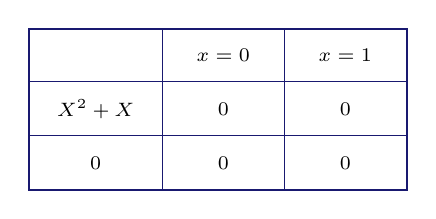
\begin{tikzpicture}[font=\scriptsize]
  \draw[MidnightBlue,thick] (0,0) rectangle (4.8,2.05);
  \draw[MidnightBlue] (1.7,0) -- (1.7,2.05);
  \draw[MidnightBlue] (3.25,0) -- (3.25,2.05);
  \draw[MidnightBlue] (0,1.38) -- (4.8,1.38);
  \draw[MidnightBlue] (0,0.69) -- (4.8,0.69);
  \node at (2.47,1.71) {$x=0$};
  \node at (4.02,1.71) {$x=1$};
  \node at (0.85,1.03) {$X^2+X$};
  \node at (2.47,1.03) {$0$};
  \node at (4.02,1.03) {$0$};
  \node at (0.85,0.34) {$0$};
  \node at (2.47,0.34) {$0$};
  \node at (4.02,0.34) {$0$};
\end{tikzpicture}
